\documentclass[
	% -- opções da classe memoir --
	12pt,				% tamanho da fonte
	%openright,			% capítulos começam em pág ímpar (insere página vazia caso preciso)
	%twoside,			% para impressão em verso e anverso. Oposto a oneside
	oneside,			% para impressão em verso e anverso. Oposto a oneside
	a4paper,			% tamanho do papel.
	% -- opções da classe abntex2 --
	%chapter=TITLE,		% títulos de capítulos convertidos em letras maiúsculas
	%section=TITLE,		% títulos de seções convertidos em letras maiúsculas
	%subsection=TITLE,	% títulos de subseções convertidos em letras maiúsculas
	%subsubsection=TITLE,% títulos de subsubseções convertidos em letras maiúsculas
	% -- opções do pacote babel --
	english,			% idioma adicional para hifenização
	brazil,				% o último idioma é o principal do documento
	% -- opções da classe ime-abntex2 --
	%brasao,
	]{ime-abntex2}


% ---
% PACOTES
% ---

% ---
% Pacotes fundamentais
% ---
\usepackage[utf8]{inputenc}		% Codificacao do documento (conversão automática dos acentos)
\usepackage{cmap}			% Mapear caracteres especiais no PDF
\usepackage{lmodern}			% Usa a fonte Latin Modern
%\usepackage{amsmath}			% Para usar fontes ams
%\usepackage{amsfonts}			% Para usar fontes ams
%\usepackage{times}			% Usa a fonte Times
\usepackage[T1]{fontenc}		% Selecao de codigos de fonte.
\usepackage{indentfirst}		% Indenta o primeiro parágrafo de cada seção.
\usepackage{color}			% Controle das cores
\usepackage{graphicx}			% Inclusão de gráficos
\usepackage{algorithm2e}		% Para escrever algorítimos
% ---

% ---
% Pacotes adicionais, usados apenas no âmbito do documento em questão
% ---
%\usepackage{lipsum}			% para geração de dummy text
% ---

% ---
% Pacotes de citações
% ---
\usepackage[brazilian,hyperpageref]{backref}	 % Paginas com as citações na bibl
\usepackage[alf]{abntex2cite}	% Citações padrão ABNT

% ---
% CONFIGURAÇÕES DE PACOTES
% ---

% ---
% Configurações do pacote backref
% Usado sem a opção hyperpageref de backref
\renewcommand{\backrefpagesname}{Citado na(s) página(s):~}
% Texto padrão antes do número das páginas
\renewcommand{\backref}{}
% Define os textos da citação
\renewcommand*{\backrefalt}[4]{
	\ifcase #1 %
		Nenhuma citação no texto.%
	\or
		Citado na página #2.%
	\else
		Citado #1 vezes nas páginas #2.%
	\fi}%
% ---


% ---
% Informações de dados para CAPA e FOLHA DE ROSTO
% ---
\titulo{Trabalho Sobre IPv6 e NAT}
\autor{
  Bruno Campana\\
  Jan Segre\\
  Jonas Amaro\\
}
\local{Rio de Janeiro}
\data{Abril de 2014}
\orientador{Maj Cardoso}
%\coorientador{Equipe \abnTeX}
\instituicao{%
  Instituto Militar de Engenharia
  \par
  Seção de Computação
  \par
  Graduação em Engenharia de Computação}
%\tipotrabalho{Iniciação à Pesquisa}
% O preambulo deve conter o tipo do trabalho, o objetivo,
% o nome da instituição e a área de concentração
%\preambulo{Iniciação à Pesquisa apresentada ao Curso de Graduação
%em Engenharia de Computação do Instituto Militar de
%Engenharia.}
% ---


% ---
% Configurações de aparência do PDF final

% alterando o aspecto da cor azul
%\definecolor{blue}{RGB}{41,5,195}
\definecolor{blue}{RGB}{0,0,0}

% informações do PDF
\makeatletter
\hypersetup{
	%pagebackref=true,
	pdftitle={\@title},
	pdfauthor={\@author},
	pdfsubject={\imprimirpreambulo},
	pdfcreator={LaTeX with abnTeX2},
	pdfkeywords={ime}{robocup}{analise}{logs}{rede neural},
	colorlinks=true,		% false: boxed links; true: colored links
	linkcolor=blue,			% color of internal links
	citecolor=blue,			% color of links to bibliography
	filecolor=magenta,		% color of file links
	urlcolor=blue,
	bookmarksdepth=4
}
\makeatother
% ---

% ---
% Espaçamentos entre linhas e parágrafos
% ---

% O tamanho do parágrafo é dado por:
%\setlength{\parindent}{1.3cm}

% Controle do espaçamento entre um parágrafo e outro:
%\setlength{\parskip}{0.2cm}  % tente também \onelineskip
\setlength{\parskip}{\onelineskip}

% ---
% compila o indice
% ---
\makeindex
% ---

% ----
% Início do documento
% ----
\begin{document}

% Retira espaço extra obsoleto entre as frases.
%\frenchspacing


% ----------------------------------------------------------
% ELEMENTOS PRÉ-TEXTUAIS
% ----------------------------------------------------------
% \pretextual

% ---
% Capa
% ---
\imprimircapa
%\input{pre_textuais/capa}
% ---

% ---
% inserir o sumario
% ---
\pdfbookmark[0]{\contentsname}{toc}
\tableofcontents*
\cleardoublepage
% ---


% ----------------------------------------------------------
% ELEMENTOS TEXTUAIS
% ----------------------------------------------------------
\textual

\chapter{Sobre IPv6}

\section{Introdução}
IPv6 foi desenvolvido para substituir o IPv4 e acabar com a ameaça de escassez de endereços. Por essa razão o IPv6 não foi preparado para funcionar em conjunto do IPv4 e sim substituí-lo. Desse modo, se planejava que a implementação do IPv6 ocorresse em double stack, ou seja que houvesse duas redes IPv4 e IPv6 simultaneamente, até que fosse mitigado o IPv4. Por diversas razões, não foi possível realizar o double stack. Como o artigo[http://www.networkworld.com/news/tech/2007/090507-tech-uodate.html] sugere, apesar da utilização de técnicas de tunelamento terem diversos problemas, elas se mostram bastante úteis para alguns casos.


\section{Cenários de coexistência IPv4 x IPv6}
- Dado que em um estado intermediário de coexistência dos dois protocolos, oito cenários foram abordados na RFC 6144, de modo que todos as técnicas de transição devem contemplar se quiserem manter a interoperabilidade no período de transição

\subsection{Da rede IPv6 para a internet IPv4}
Se uma organização decidir manter sua rede IPv6, mas ainda encontrar a internet operando em IPv4, será necessário a adaptação da fronteira dos dois protocolos. Para esse tipo de cenário, a tradução do IPv6 para o IPv4 é inevitável. Nesse caso, as solução podem ser stateful ou stateless.

\subsection{Da internet IPv4 para a rede IPv6}
Por outro lado, a interoperabilidade deve ser garantida também caso, queira-se montar um servidor IPv6 para outros usuários da rede IPv4. Nesse caso, soluções stateful, como NAT-PT, podem ser utilizadas, assim como soluções stateless, já que existe um subconjunto do IPv6 destinado para o endereçamento do IPv4.

\subsection{Da internet IPv6 para a rede IPv4}
Esse é um caso em que o domínio maior precisa ser identificado dentro de um domínio menor. Por causa disso, não é possível mapear diretamente os IPv6 que queiram acessar a rede IPv4 a menos que seja uma solução stateful.


\subsection{Rede IPv4 precisa se comunicar com internet IPv6}
Esse caso pode ocorrer por falta de recursos da organização responsável por alguma rede que utiliza IPv4, quando a implementação do novo protocolo já estiver bem sedimentada. Esse é um caso apontado como difícil pelo RFC 6144, mas que pode ser tratado pelo NAT-PT.

\subsection{Rede IPv4 precisa se comunicar com rede IPv6}
Esse caso ocorre quando uma organização tem máquinas em IPv4 e máquina em IPv6. O escopo não é muito diferente do cenário 1, por isso o tratamento dos estados é indiferente.

\subsection{Rede IPv6 precisa se comunicar com rede IPv4}
Ocorre nos mesmo caso do cenário 5 e pode ser resolvido da mesma maneira que o cenário 2.

\subsection{Internet IPv6 precisa se comunicar com internet IPv4}
Esse cenário ocorre quando o IPv6 já estiver com certa maturidade, mas o IPv4 ainda não é desprezível. Devida a grande diferença do tamanho de IPs, não existe nenhuma solução de tradução viável.

\subsection{Internet IPv4 precisa se comunicar com internet IPv6}
Se analisarmos o cenário 7 no sentido contrário da comunicação, chega-se a esse cenário e igualmente, não foi apresentado nenhuma solução viável nesse cenário.

\section{Classificação as técnicas de transição}
Segundo a página[http://ipv6.br/entenda/transicao] existem 3 tipos técnicas:

\begin{itemize}
  \item
    \textbf{Pilha Dupla}

    Nesse caso as duas redes IPv4 e IPv6 operam simultaneamente. Sua aplicação ideal ocorre quando se fornece IPv6 e IPv4 para todas as máquinas

  \item
    \textbf{Túneis}

    Permite o transito de informação de ilhas IPv6, ou IPv4, em oceano IPv4, ou IPv6.

  \item
    \textbf{Tradução}

    A comunicação máquinas que rodam protocolos IP diferentes é viabilizada.
\end{itemize}


\chapter{Sobre NAT}

\section{O desenvolvimento do protocolo NAT}

Em meados do meio da década de 90, já vislumbrava-se que em breve o protocolo de endereçamento IPv4
chegaria a sua exaustão, e não haveriam mais endereços livres para serem distribuídos a novos dispositivos.
Buscou-se então o desenvolvimento de uma solução de rápida implementação e que não envolvesse toda uma
troca do padrão de endereçamento corrente, ainda que fosse temporária. É nesse cenário que ocorreu a
implementação e popularização do protocolo NAT, Network Address Translation, que consiste em um mecanismo
que permite o compartilhamento de um mesmo endereço IP por vários hosts para acesso à internet.

\section{Como NAT opera}

Supondo uma rede interna com vários hosts, e com apenas um endereço de IP válido na web disponível,
implementa-se o protocolo NAT para que todas as máquinas possam acessar a internet de modo transparente
à aplicação. Um host dessa rede interna possui um endereço IP de uso local, não-válido na web.
Ao enviar um pacote, esse host irá endereçá-lo com seu endereço IP não-válido. Todos os pacotes
dessa rede interna com destinatário externo passarão pelo roteador que estará operando o protocolo NAT.
Dessa forma, fazendo uso de uma tabela de tradução direta, o roteador substitui o IP não-válido do host
fonte pelo seu próprio, válido na internet. Em seguida, os pacotes que porventura
cheguem como resposta do destinatário terão seu IP destino substituído novamente nesse roteador pelo IP que originalmente fez a requisição.

%! FIGURA: Single_NAT
\begin{figure}[ht]
\centering
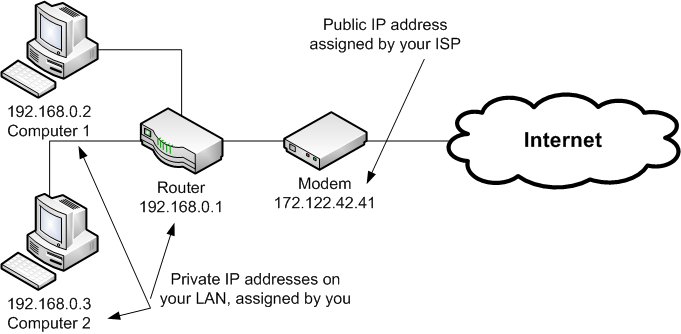
\includegraphics[width=10cm]{imgs/Single_NAT}
%\caption{descricao}\label{fig:single_nat}
\end{figure}

\subsection{Funcionamento da tradução de endereços}

No que diz respeito a formatação da tabela de endereços e a forma como a tradução ocorre, temos as três
possíveis configurações que seguem.

\subsubsection{Utilizando um único endereço IP}

Nesse formato, o endereço IP dos remetentes possui uma única possibilidade de substituição, conforme
descrito no exemplo de "2 Como NAT opera". A tabela de tradução consiste em duas colunas, uma para IP remetente e outra para IP
destino.

\subsubsection{Utilizando um pool de endereços IP}

Se toda uma rede local depende de um único endereço IP válido para acessar a internet, existe a limitação
de que dois hosts não podem trocar pacotes com o mesmo destinatário, pois ao receber um pacote externo nessa
situação, o roteador NAT não saberia a qual dos dois hosts este pertente. Para resolver esse problema, o roteador
NAT usa um pool de endereços. Nessa situação a tabela de tradução possui as mesmas duas colunas.

\subsubsection{Uso simultâneo de endereço IP e número de porta}

Uma outra forma menos restritiva de estender a troca de pacotes de vários hosts na mesma rede interna com um
mesmo host externo consiste na tabela de tradução conter três colunas adicionais, uma para cada endereço de porta
e uma para o protocolo empregado. Dessa forma é possível na prática que qualquer quantidade de hosts de uma rede interna
troque pacotes com um mesmo host da rede interna pelo mesmo endereço de IP. Essa variação do protocolo NAT é chama-se
NAPT, porém é indistintamente também chamado de NAT. Em seguida, iremos nos aprofundar melhor na operação do NAT
deixando subetendido o uso deste terceiro método todo o tempo.

\section{Formas de implementação do NAT}

No tópico anterior, a abordagem de nossa explicação deixa implícito que estamos tratanto de uma troca de
pacotes iniciada pelo host interno, afinal, não é possível para um host externo iniciar uma troca de pacotes, uma vez que
tudo que ele pode saber sobre os hosts naquela rede é o endereço IP do Gateway. Uma vez que o mapeamento entre
dois endereços ocorra (um interno e um externo), ainda resta definir como ocorrerá o emprego do endereçamento de
portas. A seguir, veremos as quatro formas pelas quais pode ocorrer o endereçamento de portas do NAT.


\subsection{Symmetric}

Nesta forma de comportamento, a troca de pacotes ocorre estritamente entre os conjuntos de endereço IP
e de porta interno e externo que estão na ligação. Não pode ocorrer por exemplo, de durante a ligação de um
cliente interno e um servidor externo, que um segundo servidor realiza a entrega de um pacote ao cliente.
Esse comportamento é o mais restritivo de todos e é cada vez mais raro, uma vez que impede as aplicações
de realizarem encaminhamentos, como o exemplificado.

%! FIGURA: 600px-Symmetric_NAT.svg
\begin{figure}[ht]
\centering
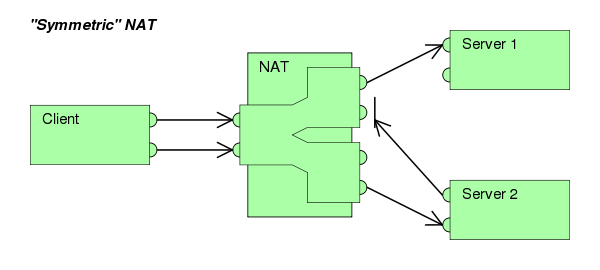
\includegraphics[width=10cm]{imgs/600px-Symmetric_NAT}
%\caption{descricao}\label{fig:single_nat}
\end{figure}

\subsection{Full-Cone}

É a forma menos restritiva de comportamento, aonde uma vez estabelecida a conexão entre um conjunto de endereço
interno e externo, permite a qualquer outro host externo pode fazer uso da ligação.

%! FIGURA: full_cone
\begin{figure}[ht]
\centering
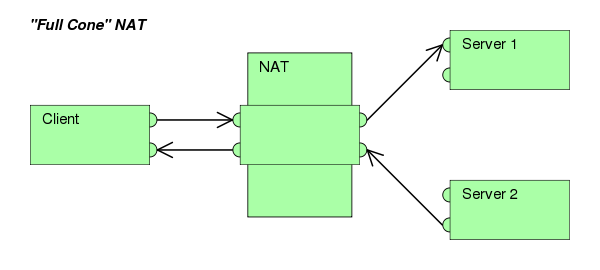
\includegraphics[width=10cm]{imgs/full_cone}
%\caption{descricao}\label{fig:single_nat}
\end{figure}

\subsection{Restricted-Cone}

Neste comportamento, apenas o host externo que fez a ligação com o conjunto de endereço interno pode enviar
pacotes, porém ele o faz empregando qualquer  uma de suas portas.

%! FIGURA: 600px-Restricted_Cone_NAT.svg
\begin{figure}[ht]
\centering
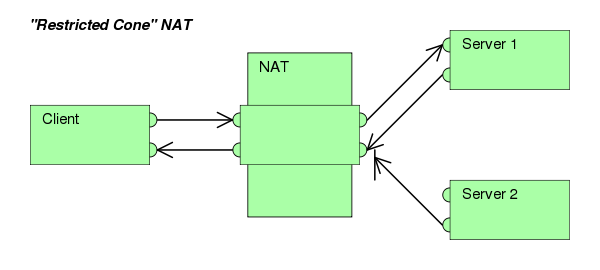
\includegraphics[width=10cm]{imgs/600px-Restricted_Cone_NAT}
%\caption{descricao}\label{fig:single_nat}
\end{figure}

\subsection{Port-Restricted-Cone}

E por fim, este comportamento permite a qualquer host externo enviar pacotes ao interno,
contanto que para isso use a mesma porta com a qual a ligação foi feita.

%! FIGURA: 600px-Port_Restricted_Cone_NAT.svg
\begin{figure}[ht]
\centering
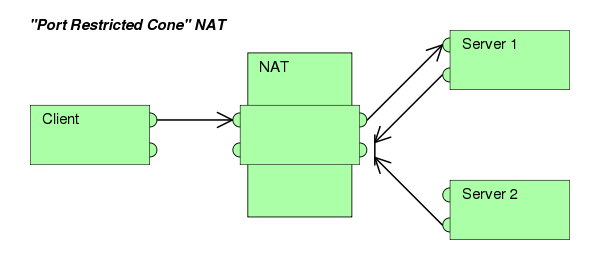
\includegraphics[width=10cm]{imgs/600px-Port_Restricted_Cone_NAT}
%\caption{descricao}\label{fig:single_nat}
\end{figure}

\section{Efeitos colaterais do NAT}

\subsection{Efeitos do NAT no endereçamento IP}

O endereçamento IP foi concebido para ser a identidade de um host na internet. Com o
compartilhamento de IPs válidos, perde-se essa característica. Perde-se segurança no nível
de camada de rede, ao passo que não há como identificar diretamente o host que enviou
determinado pacote.

\subsection{Efeitos do NAT para as aplicações}

Conforme já descrito, ficou claro que o protocolo NAT não trabalha bem quando o iniciante
da ligação encontra-se "de fora" da rede operada com NAT. Na prática, o NAT acaba por ser
um limitador ao desenvolvimento e sobrevida de aplicações, de forma a não se popularizarem aquelas
que não consigam trabalhar com ele. Aplicações que usam arquitetura peer-to-peer são as que mais
são afetadas, e acabam sendo mais complexas e frágeis.

Não obstante, a grande variedade de comportamentos e formas de implementar o NAT torna difícil
para as aplicações realizarem a predição de como proceder, e como trata-se de um protocolo
transparente (o que de modo geral é uma de suas maiores vantagens), as aplicações foi necessário
que fossem desenvolvidos métodos investigativos para as aplicações descobrirem se há um ou mais
roteadores implementando NAT no meio do caminho até o host de destino, e como estes foram implementados.

\section{Considerações finais}

Ainda que controverso, devido a série de pontos negativos citados, o protocolo NAT foi a
solução tecnológica que encontrou-se à época de forma a manter a compatibilidade com o IPv4, resolver
rapidamente o problema da escassez de endereços, sem haver neccessidade de profundas alterações
na estruturação geral da rede mundial de computadores, mudanças nos aplicativos locais ou dispositivos.

A despeito das críticas no que tange a reduzir a segurança pela introdução de "hosts fantasmas"
na rede (hosts que não possuem IP válido), o NAT introduziu novos mecanismos de segurança, a partir do
momento em que o administrador da rede ganhou controle sobre a forma como as transações podem ocorrer.

% ---
% Finaliza a parte no bookmark do PDF, para que se inicie o bookmark na raiz
% ---
\bookmarksetup{startatroot}%
% ---

% ----------------------------------------------------------
% ELEMENTOS PÓS-TEXTUAIS
% ----------------------------------------------------------
\postextual


% ----------------------------------------------------------
% Referências bibliográficas
% ----------------------------------------------------------
%\bibliographystyle{plainnat}%abbrvnat, unsrtnat, apsrev, rmpaps, IEEEtranN, achemso, rsc
%\bibliography{referencias}

\end{document}
% vim: et sw=2 ts=2 sts=2 ai si
